%%%%%%%%%%%%%%%%%%%%%%%%%%%%%%%%%%%%%%%%%%%%%%%%%%%%%%%%%%%%%%%%%%%%%%%%%%%%%%%%%%%%%%%%%%%%%%
%%                                      Inicios de la IA                                    %%
%%%%%%%%%%%%%%%%%%%%%%%%%%%%%%%%%%%%%%%%%%%%%%%%%%%%%%%%%%%%%%%%%%%%%%%%%%%%%%%%%%%%%%%%%%%%%%

\begin{frame}[fragile]{Inicios IA}
	\vspace{10px}
	\pause
	\metroset{block=fill}
	\begin{block}{Laboratorios de IA}
		\begin{itemize}
			\item SRI: Shakey, A*, ARPANET.
			\pause
			\item Laboratorio de IA del MIT: McCarthy (Lisp) y Stallman.
			\pause
			\item Robotics Institute: Sandstorm y Highlander.
		\end{itemize}
	\end{block}
	\begin{figure}
		\centering
		\pause
		\begin{subfigure}{0.33\textwidth}
			\centering
			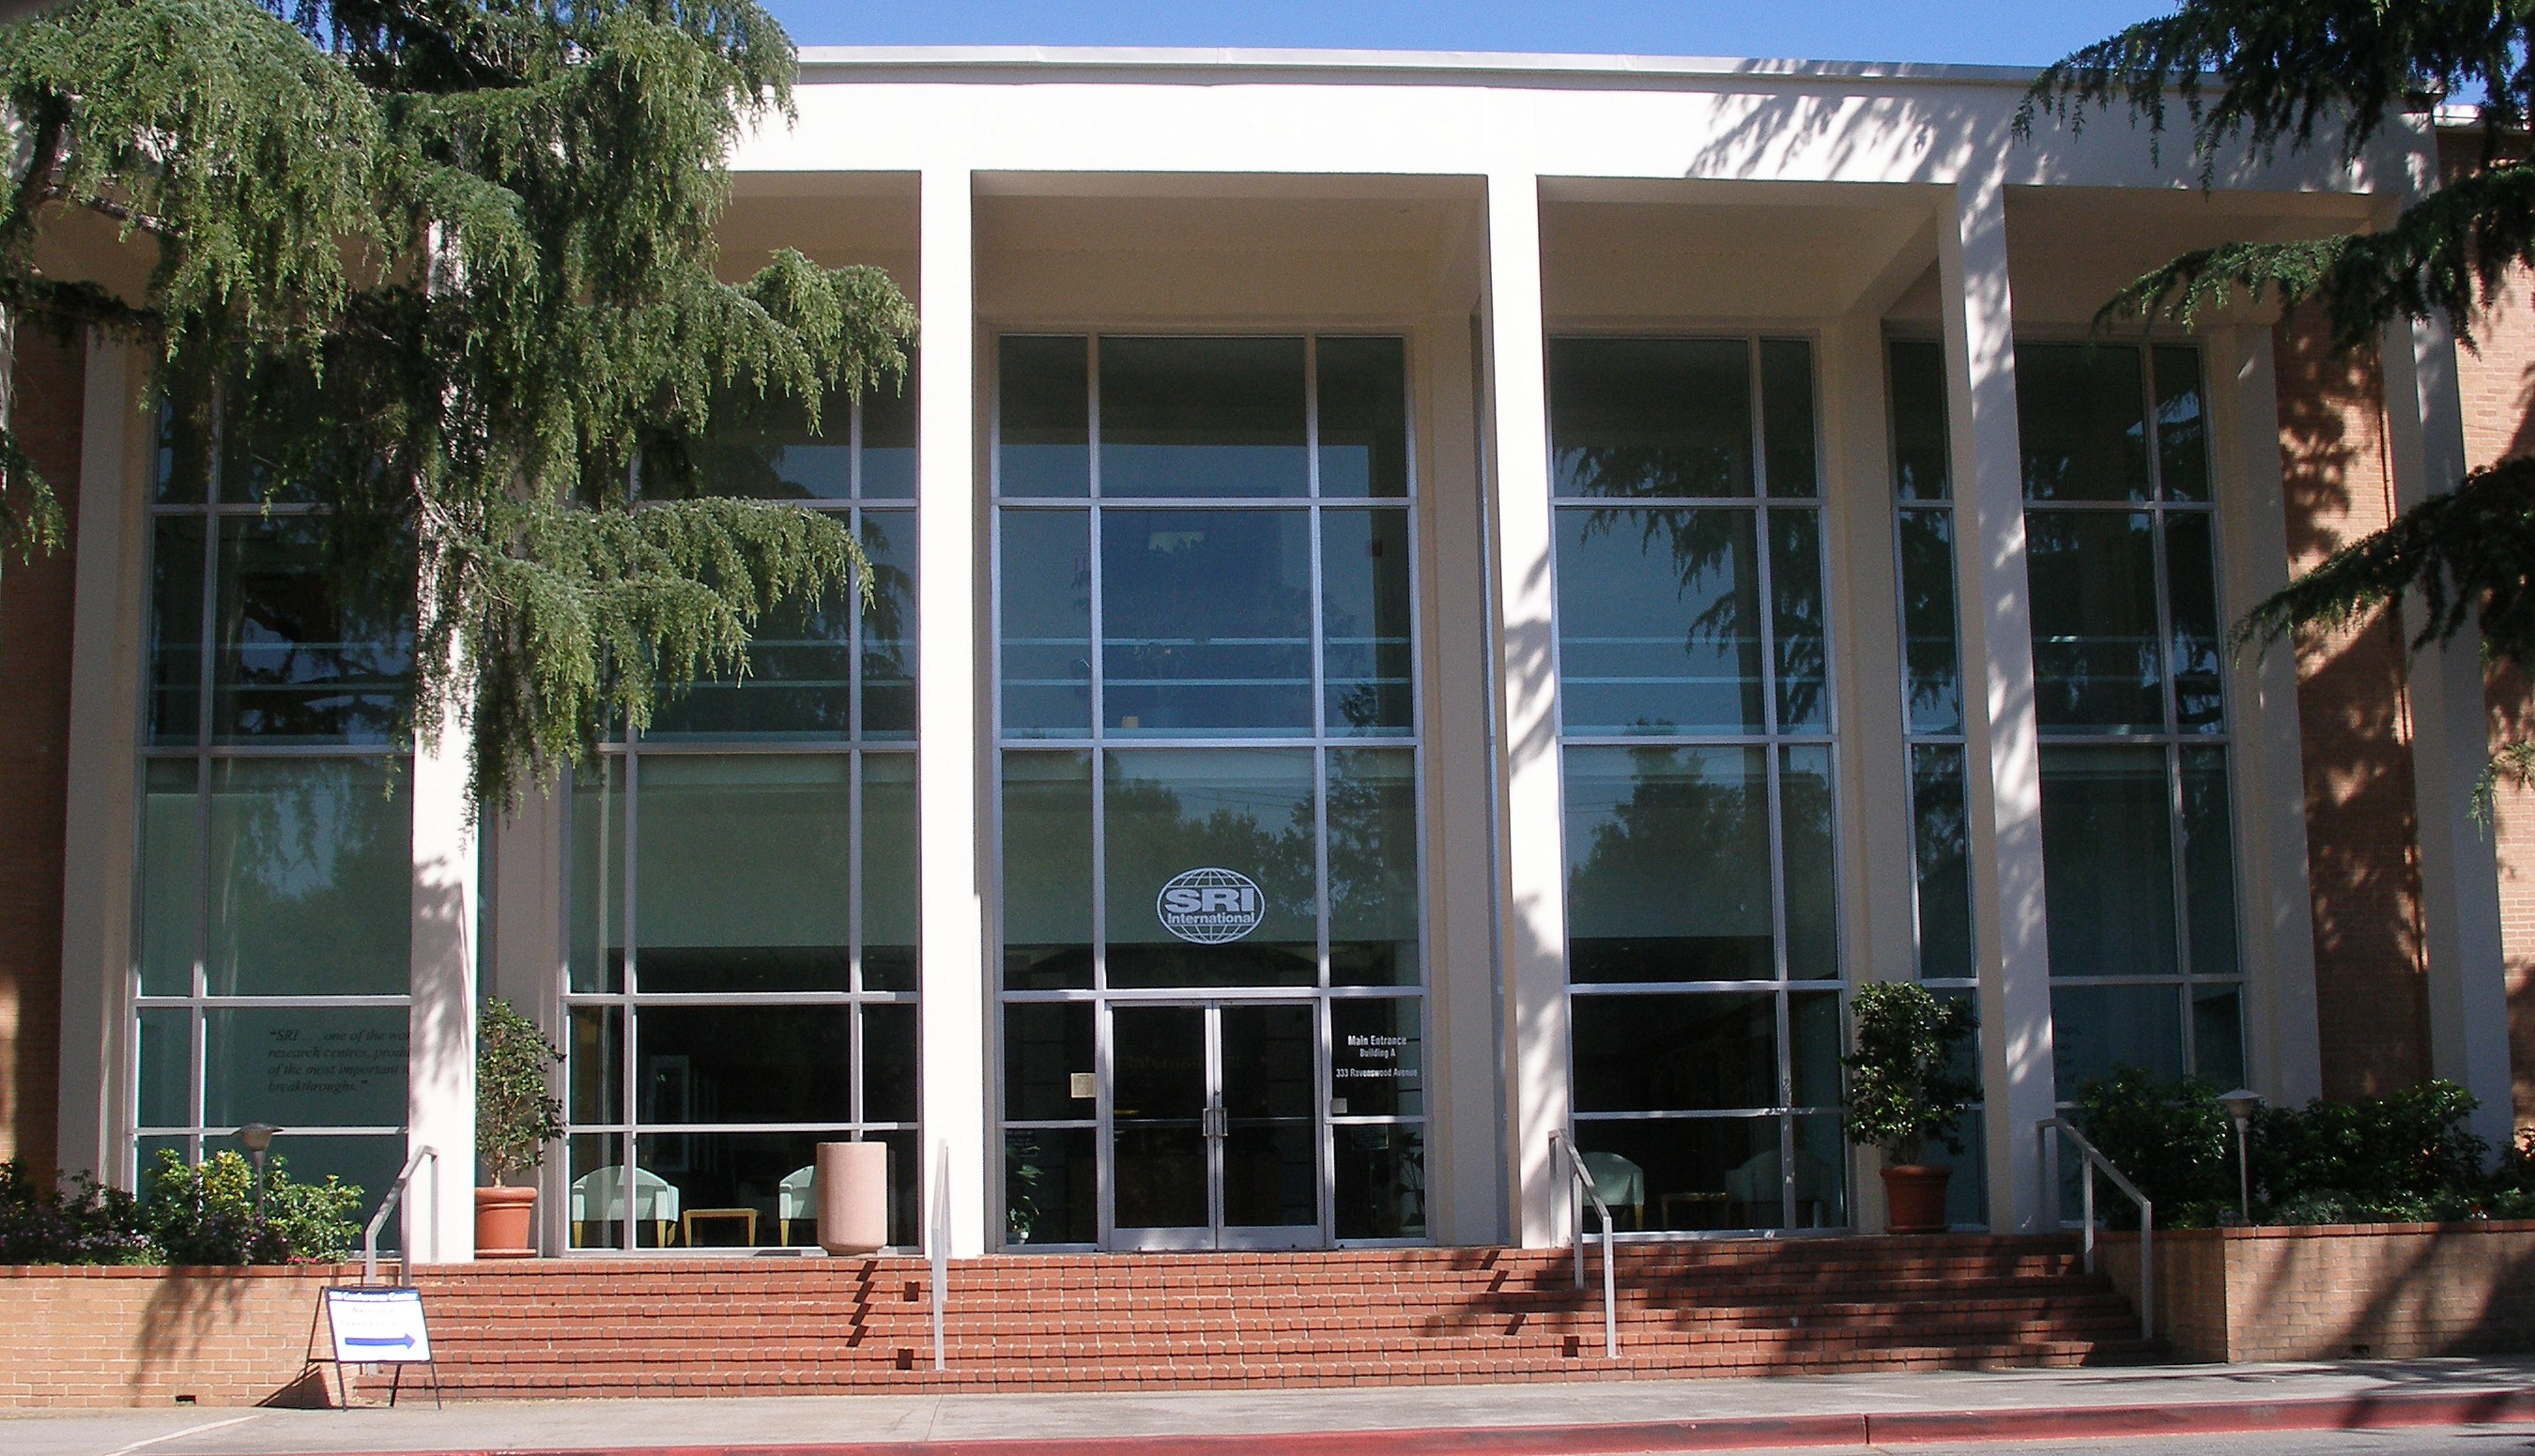
\includegraphics[scale=0.038]{./EtapaModerna/Imagenes/sri.jpg}
			\caption{SRI \href{https://es.m.wikipedia.org/wiki/Archivo:SRI_International_HQ.jpg}{Wikimedia}}
		\end{subfigure}
		\pause
		\begin{subfigure}{0.32\textwidth}
			\centering
			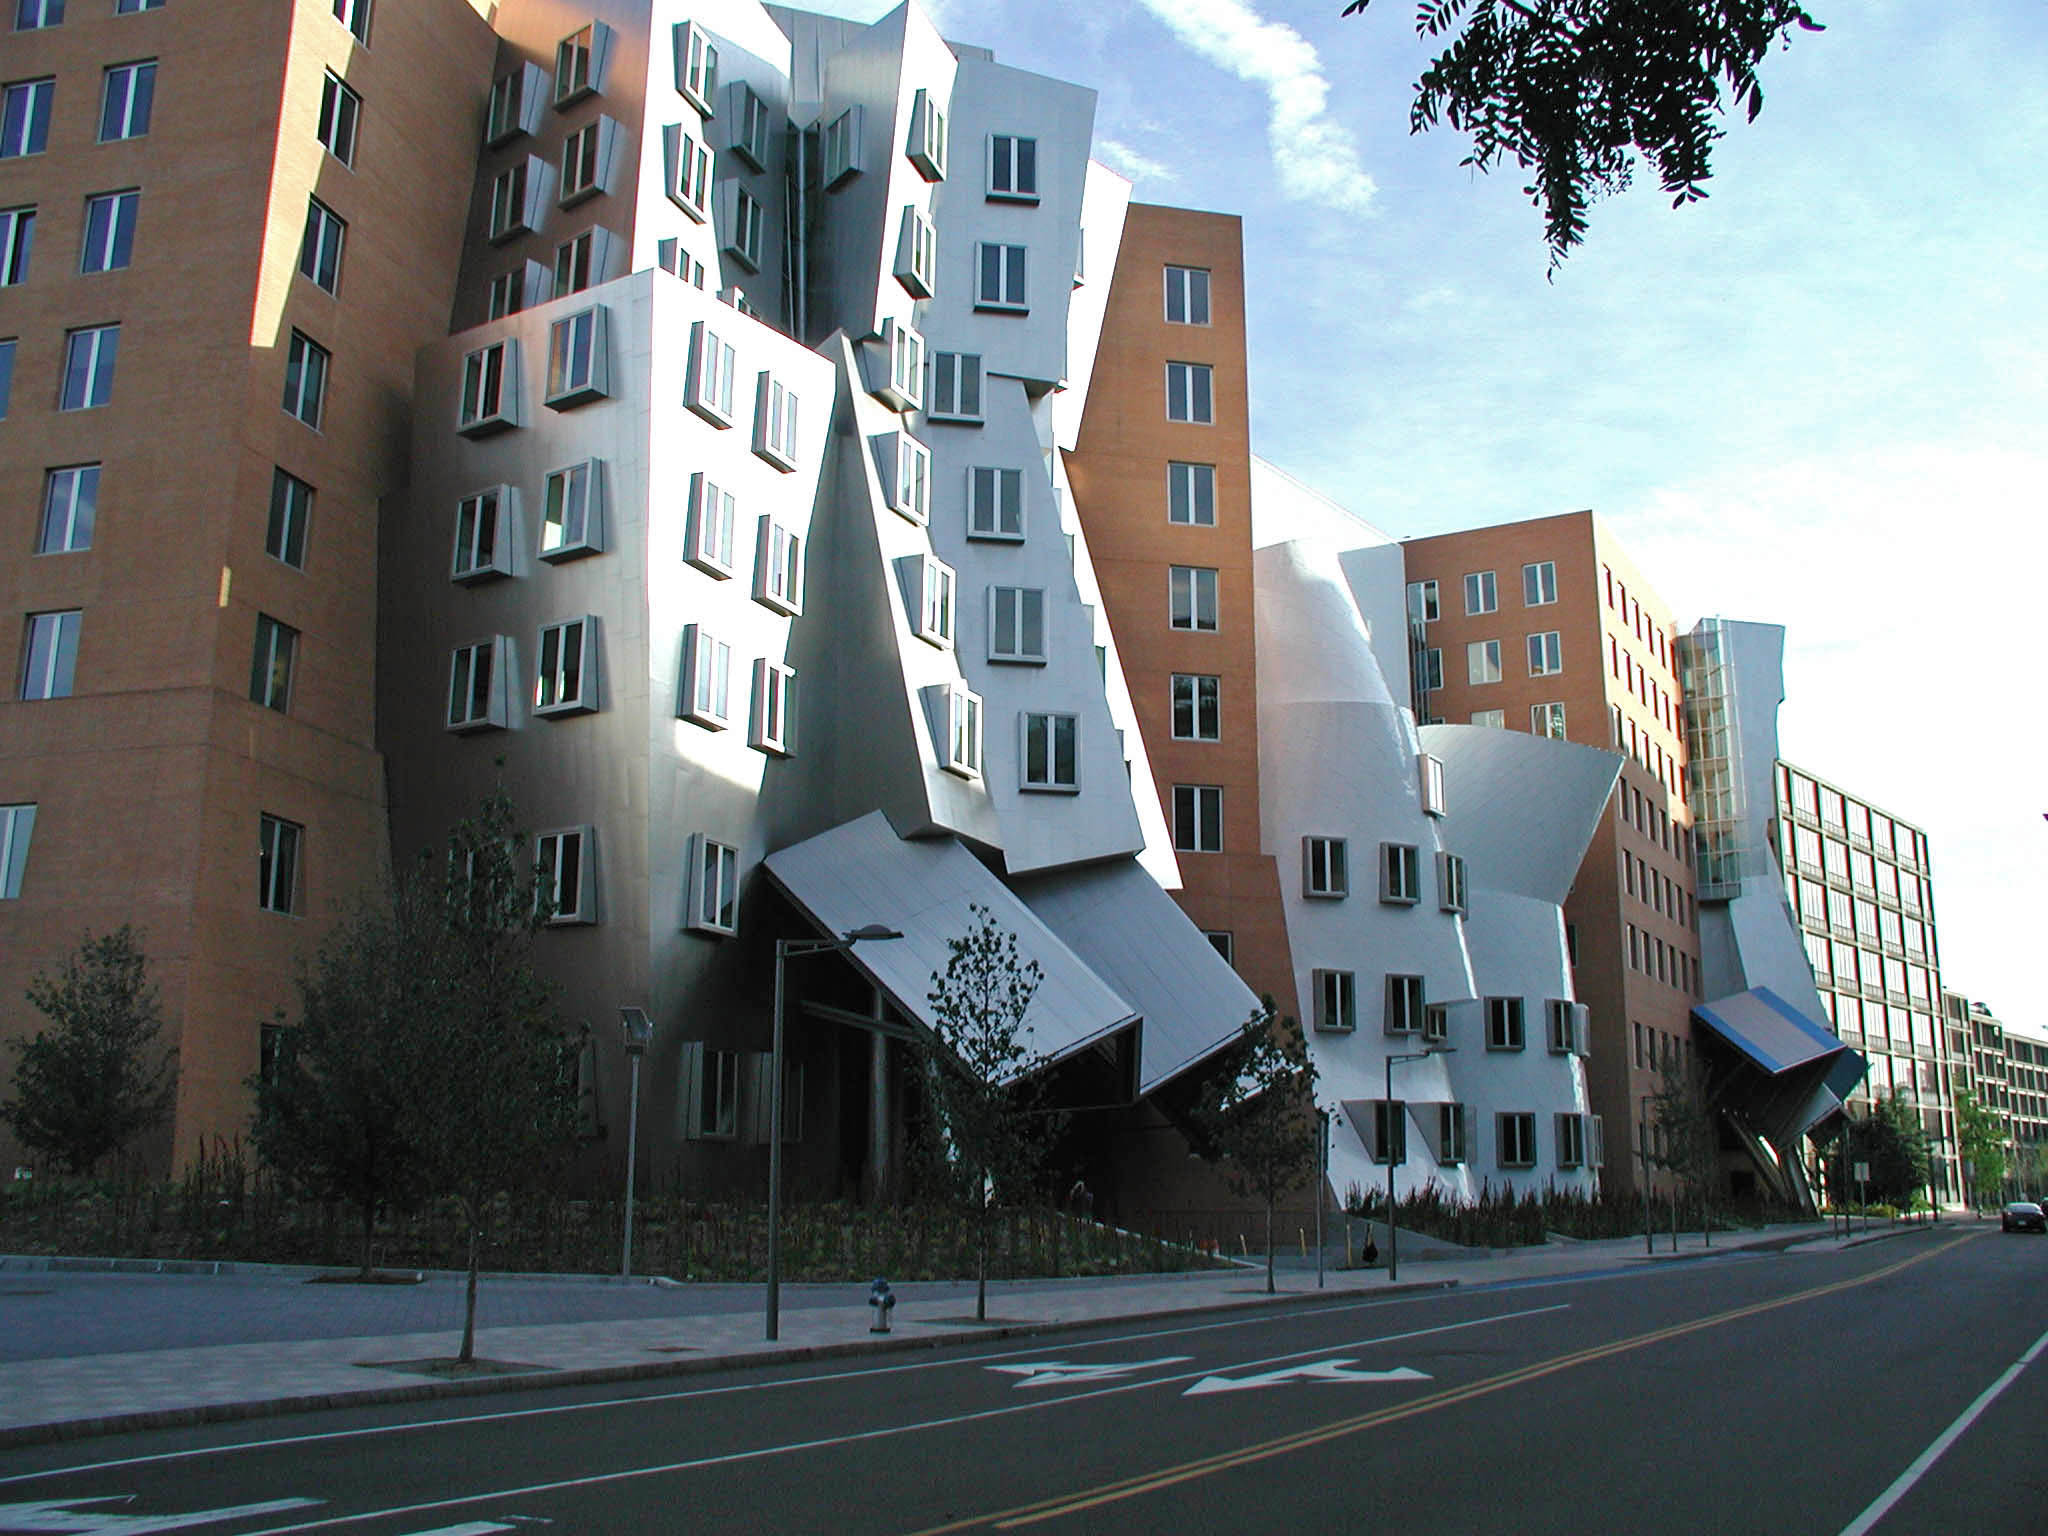
\includegraphics[scale=0.04]{./EtapaModerna/Imagenes/mit_ai.jpg}
			\caption{MIT AI Lab \href{https://commons.wikimedia.org/wiki/File:Stata_Center1.jpg}{Wikimedia}}
		\end{subfigure}
		\pause
		\begin{subfigure}{0.33\textwidth}
			\centering
			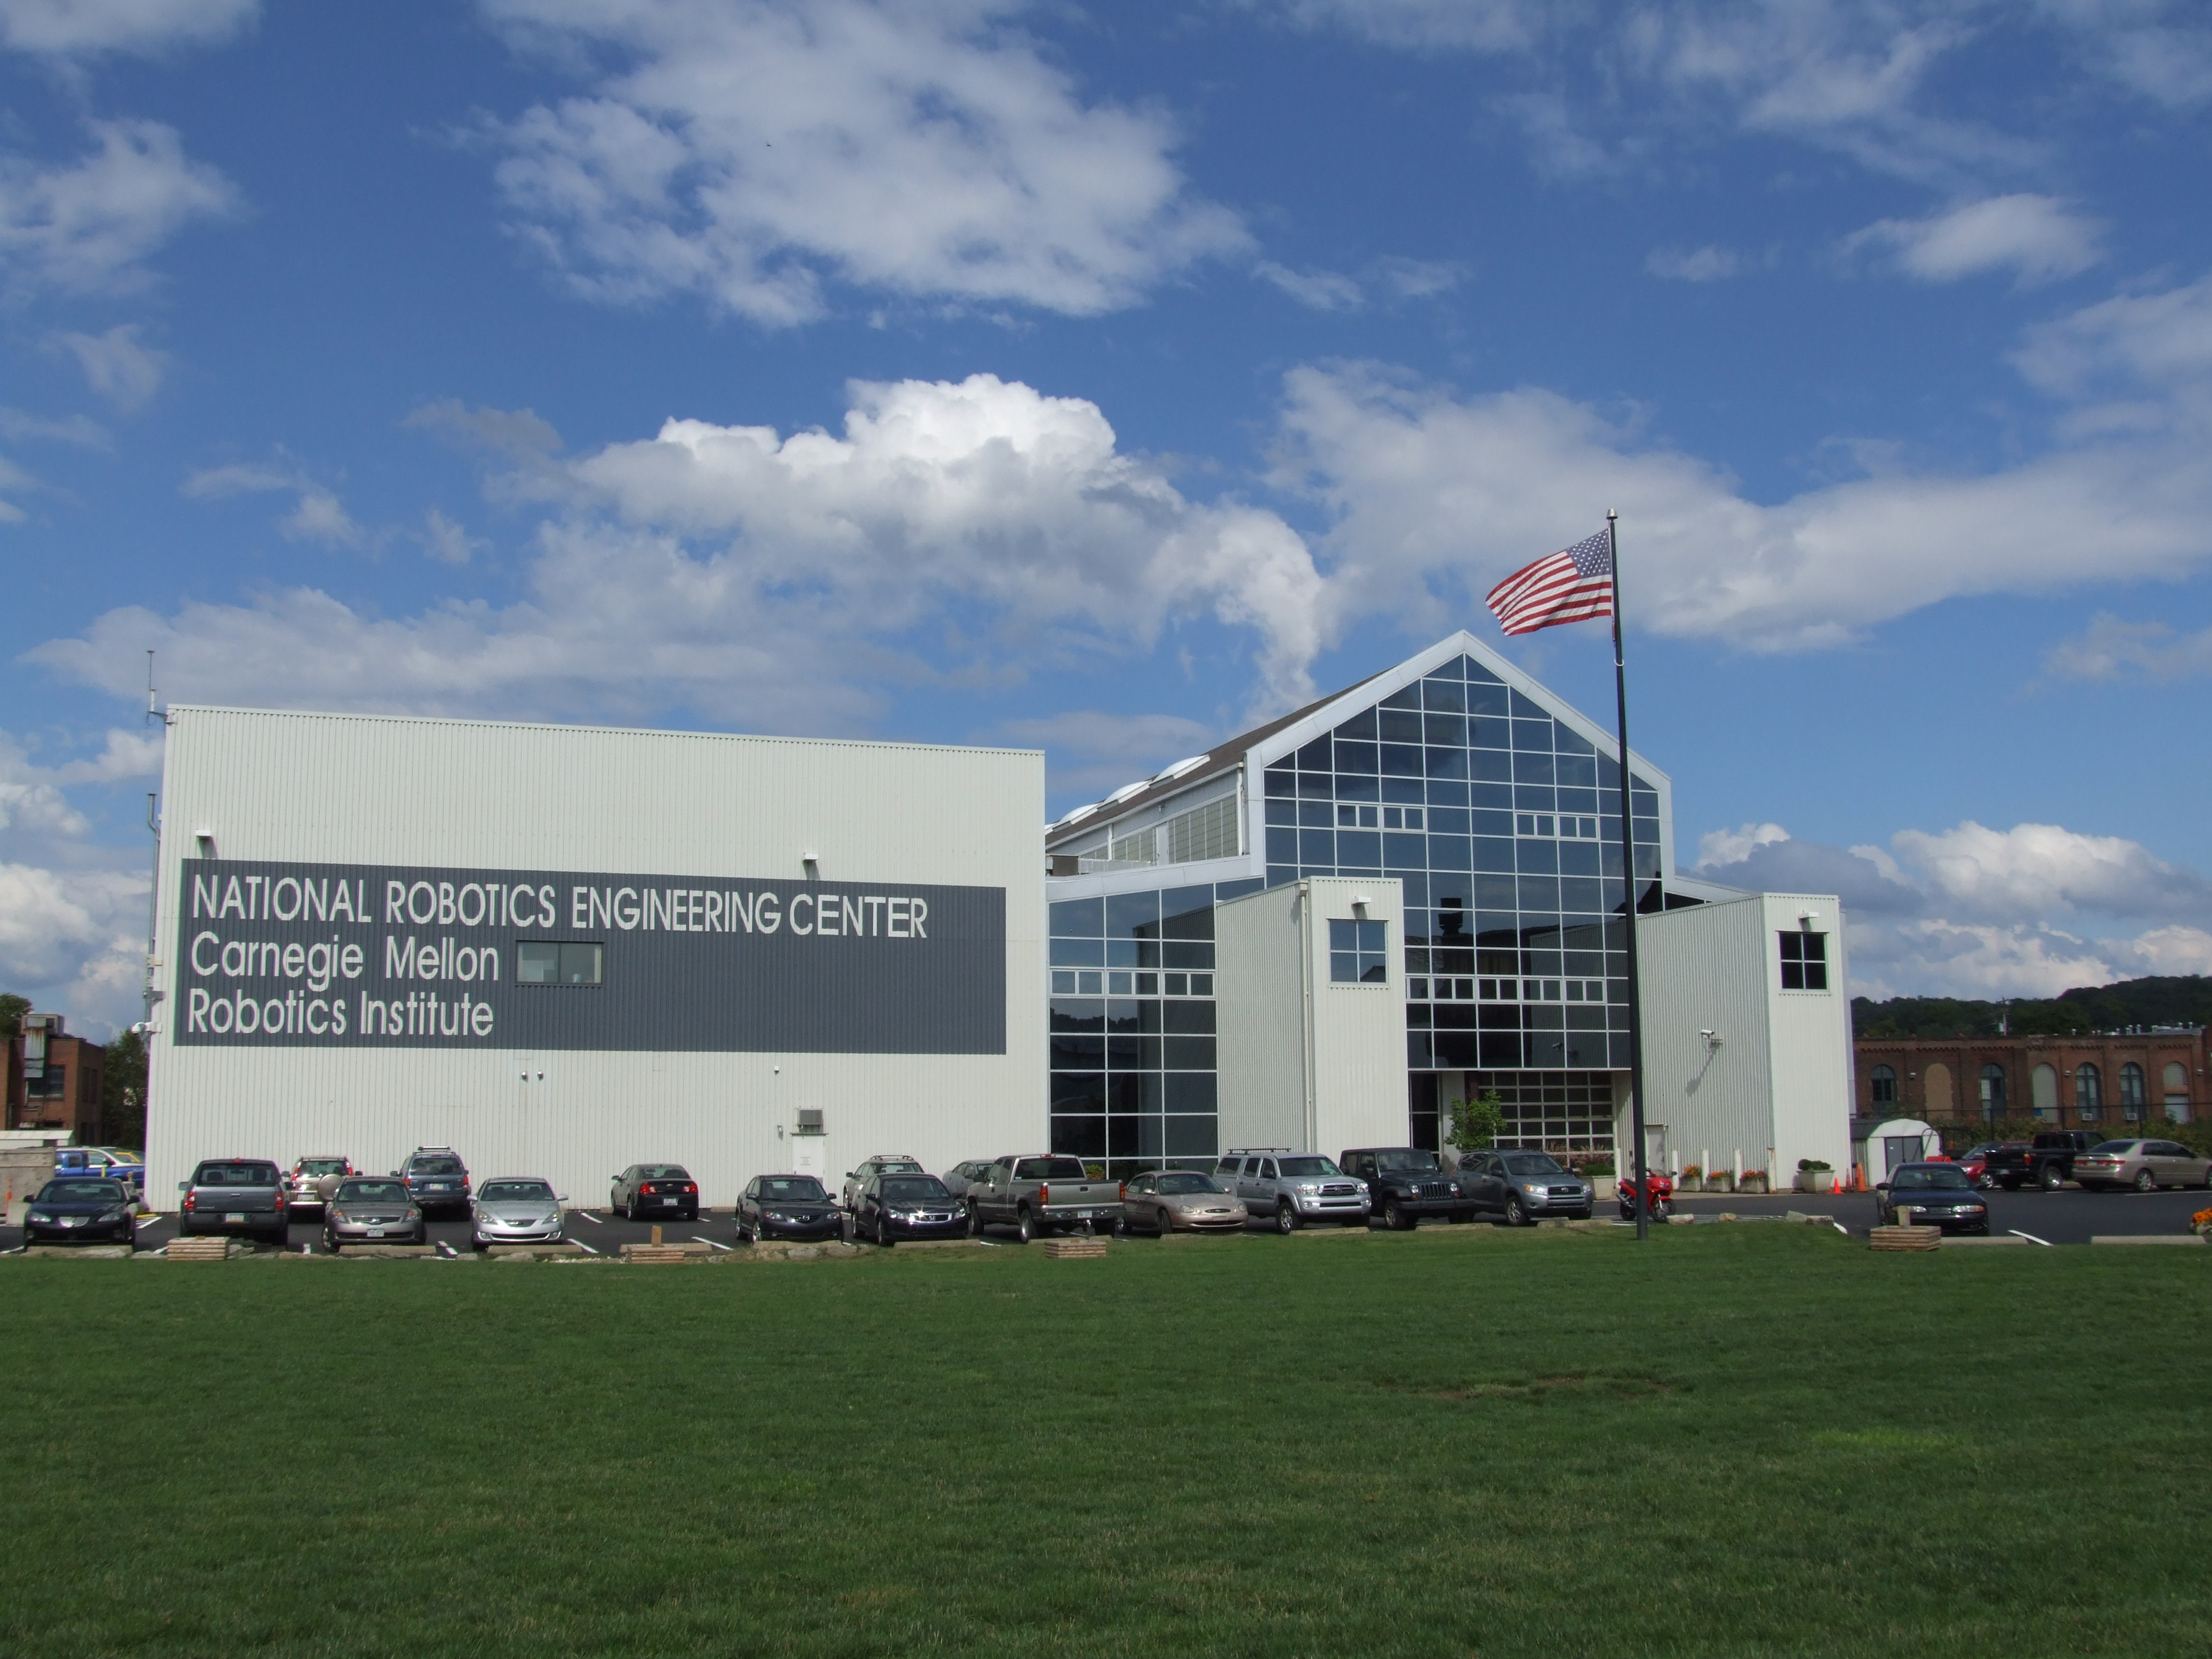
\includegraphics[scale=0.026]{./EtapaModerna/Imagenes/robotics_institute.jpg}
			\caption{Robotics Institute \href{https://commons.wikimedia.org/wiki/File:National_Robotics_Engineering_Center.JPG}{Wikimedia}}
		\end{subfigure}
	\end{figure}
\end{frame}

%%%%%%%%%%%%%%%%%%%%%%%%%%%%%%%%%%%%%%%%%%%%%%%%%%%%%%%%%%%%%%%%%%%%%%%%%%%%%%%%%%%%%%%%%%%%%%
%%                                     Brazos Robóticos                                     %%
%%%%%%%%%%%%%%%%%%%%%%%%%%%%%%%%%%%%%%%%%%%%%%%%%%%%%%%%%%%%%%%%%%%%%%%%%%%%%%%%%%%%%%%%%%%%%%

\begin{frame}[fragile]{Brazos Robóticos}
\vspace{10px}
\pause
\metroset{block=fill}
\begin{block}{Brazos Robóticos}
	\begin{itemize}
		\item Stanford Arm: eléctrico con 6 grados de libertad.
		\pause
		\item PUMA: programable fabricado por General Motors.
		\pause
		\item SCARA: primer brazo con giro en el eje Z.
	\end{itemize}
\end{block}
\begin{figure}
	\centering
	\pause
	\begin{subfigure}{0.33\textwidth}
		\centering
		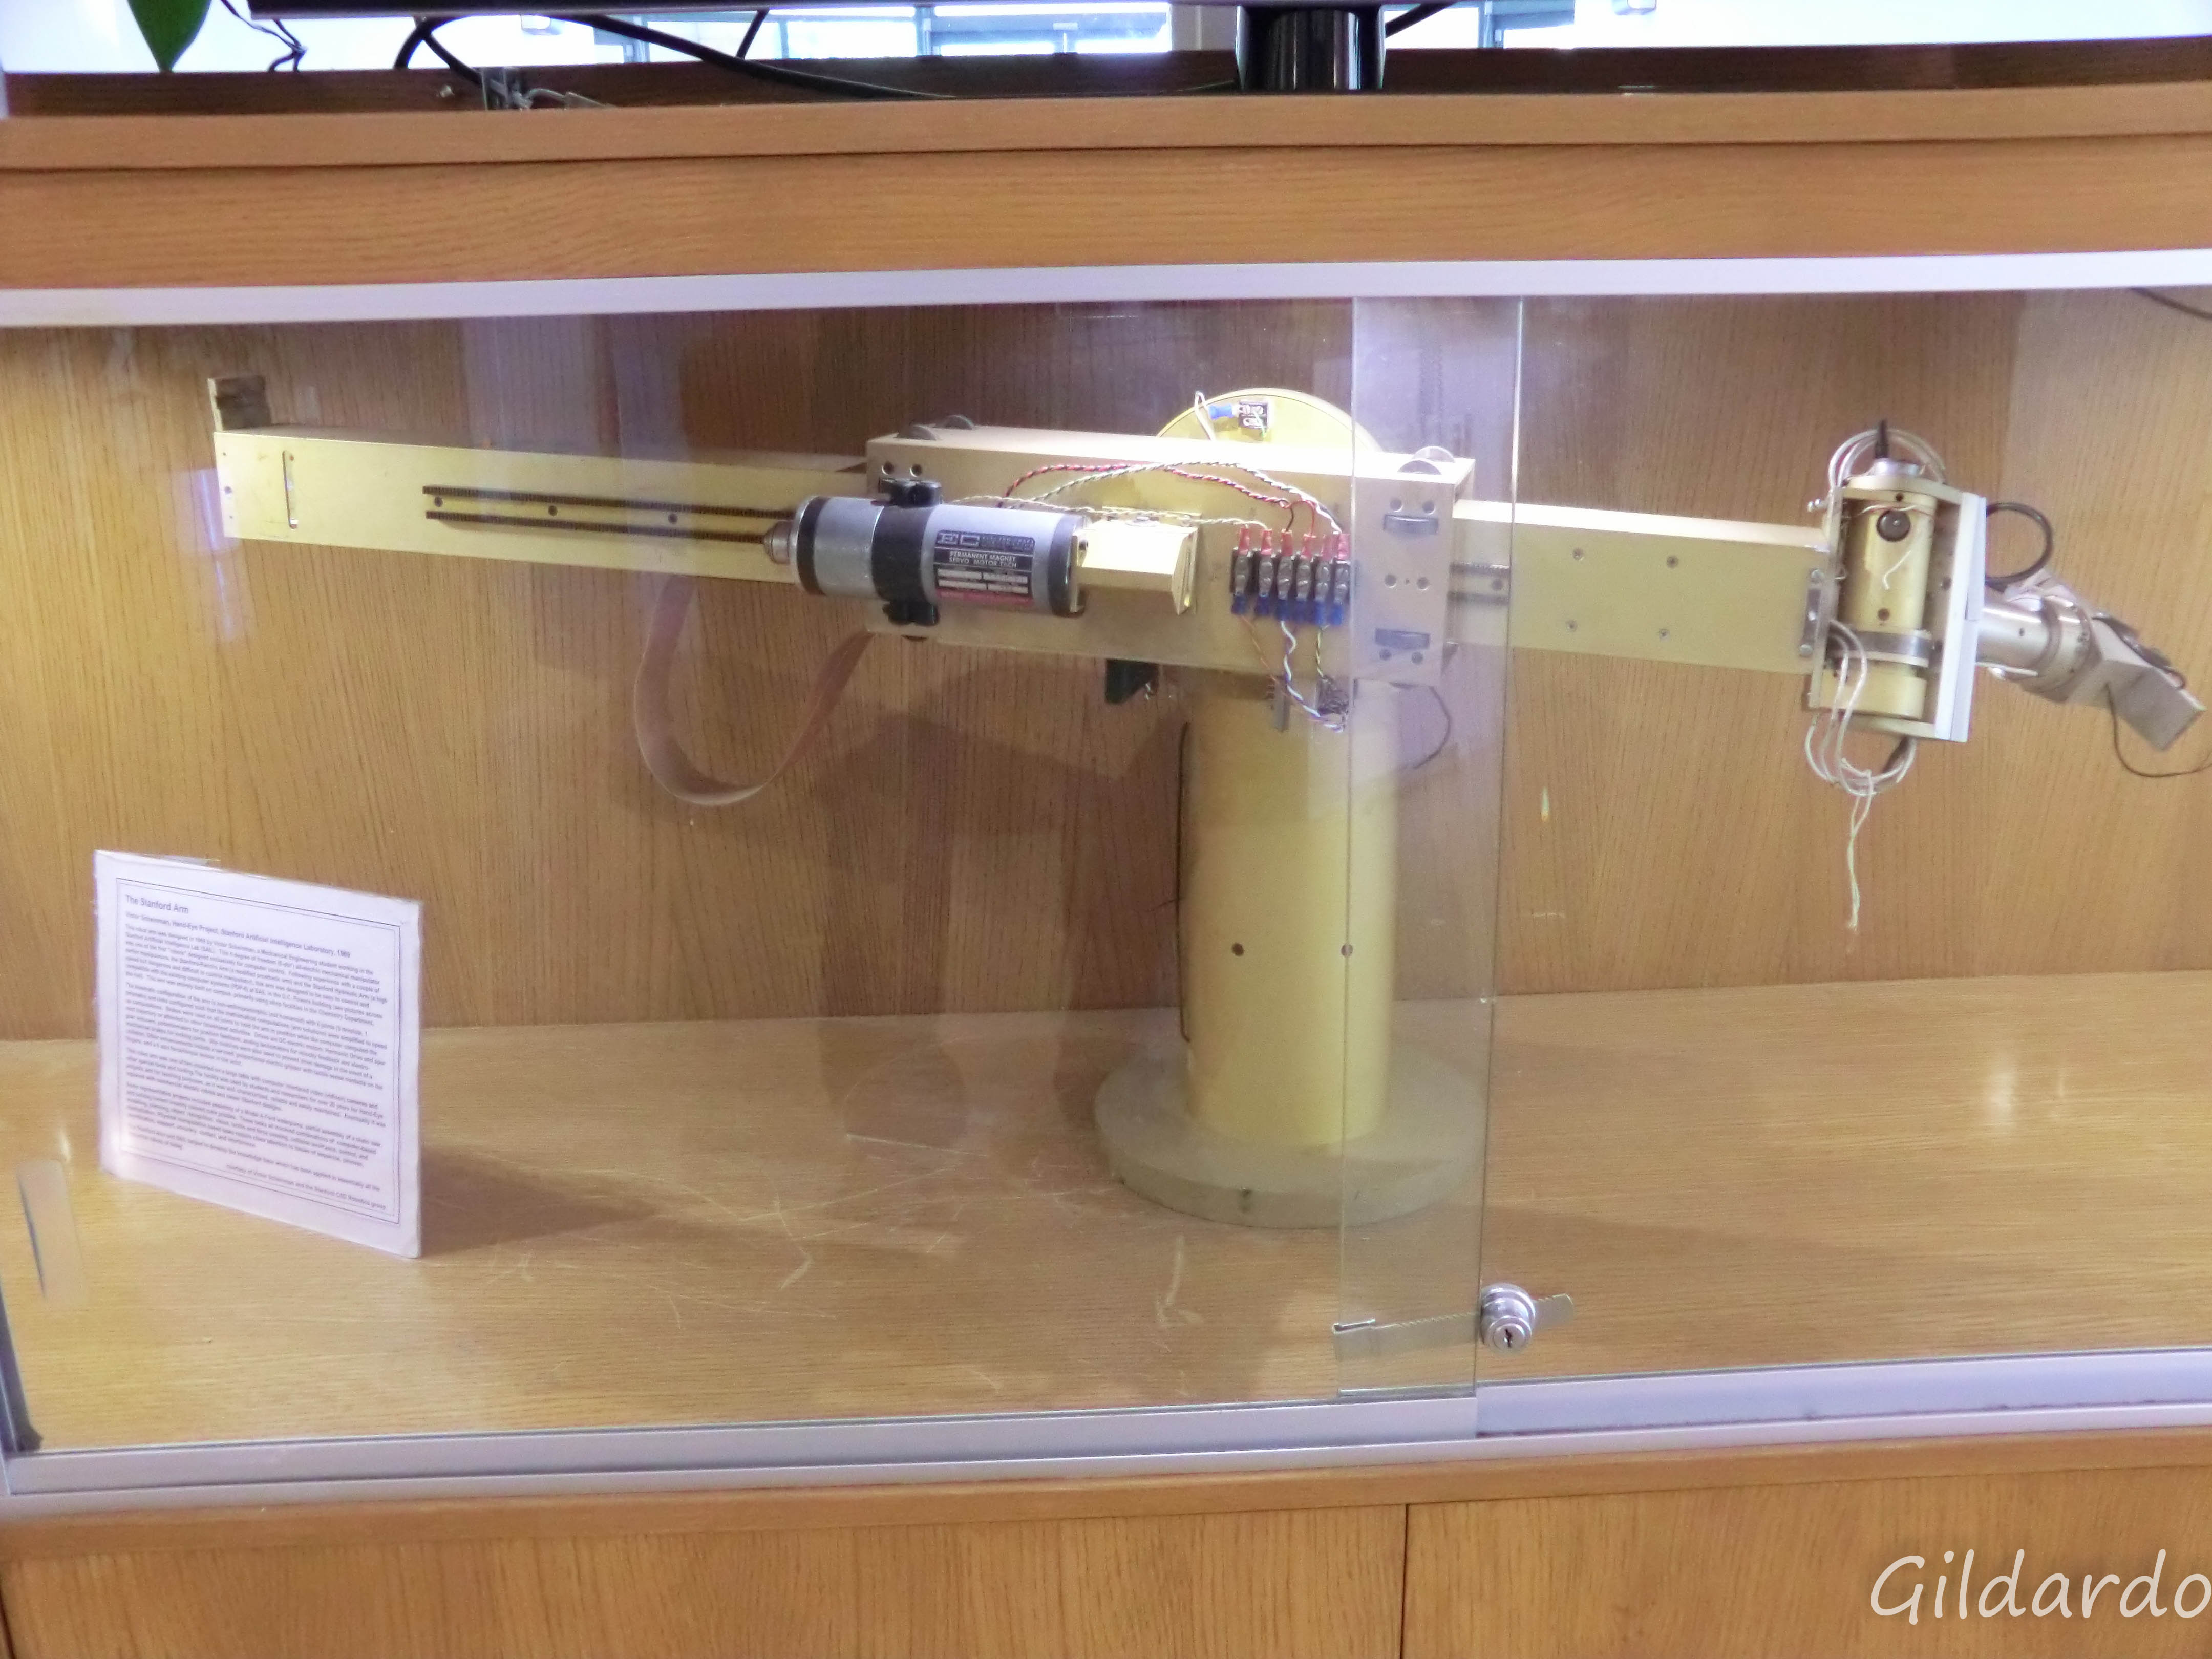
\includegraphics[scale=0.08]{./EtapaModerna/Imagenes/stanford_arm.jpg}
		\caption{Stanford Arm \href{https://www.flickr.com/photos/gildardo/6186967797}{Flickr}}
	\end{subfigure}
	\pause
	\begin{subfigure}{0.32\textwidth}
		\centering
		\includegraphics[scale=0.12]{./EtapaModerna/Imagenes/puma.jpg}
		\caption{PUMA \href{https://es.m.wikipedia.org/wiki/Archivo:Puma_Robotic_Arm_-_GPN-2000-001817.jpg}{Wikimedia}}
	\end{subfigure}
	\pause
	\begin{subfigure}{0.33\textwidth}
		\centering
		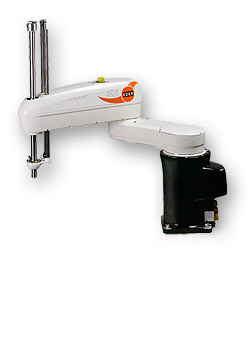
\includegraphics[scale=0.3]{./EtapaModerna/Imagenes/SCARA.jpg}
		\caption{SCARA \href{https://commons.wikimedia.org/wiki/File:KUKA_Industrial_Robot_KR10_SCARA.jpg}{Wikimedia}}
	\end{subfigure}
\end{figure}
\end{frame}

%%%%%%%%%%%%%%%%%%%%%%%%%%%%%%%%%%%%%%%%%%%%%%%%%%%%%%%%%%%%%%%%%%%%%%%%%%%%%%%%%%%%%%%%%%%%%%
%%                                        Movimiento                                        %%
%%%%%%%%%%%%%%%%%%%%%%%%%%%%%%%%%%%%%%%%%%%%%%%%%%%%%%%%%%%%%%%%%%%%%%%%%%%%%%%%%%%%%%%%%%%%%%

\begin{frame}[fragile]{Movimiento}
\vspace{10px}
\pause
\metroset{block=fill}
\begin{block}{Avance en el movimiento}
	\begin{itemize}
		\item Antecesores: RB5X, Phony Pony, WAP, Aquarobot, ...
		\pause
		\item ASIMO: \href{https://www.youtube.com/watch?v=mI58DU1hu14}{Vídeo}
	\end{itemize}
\end{block}
\begin{figure}
	\centering
	\pause
	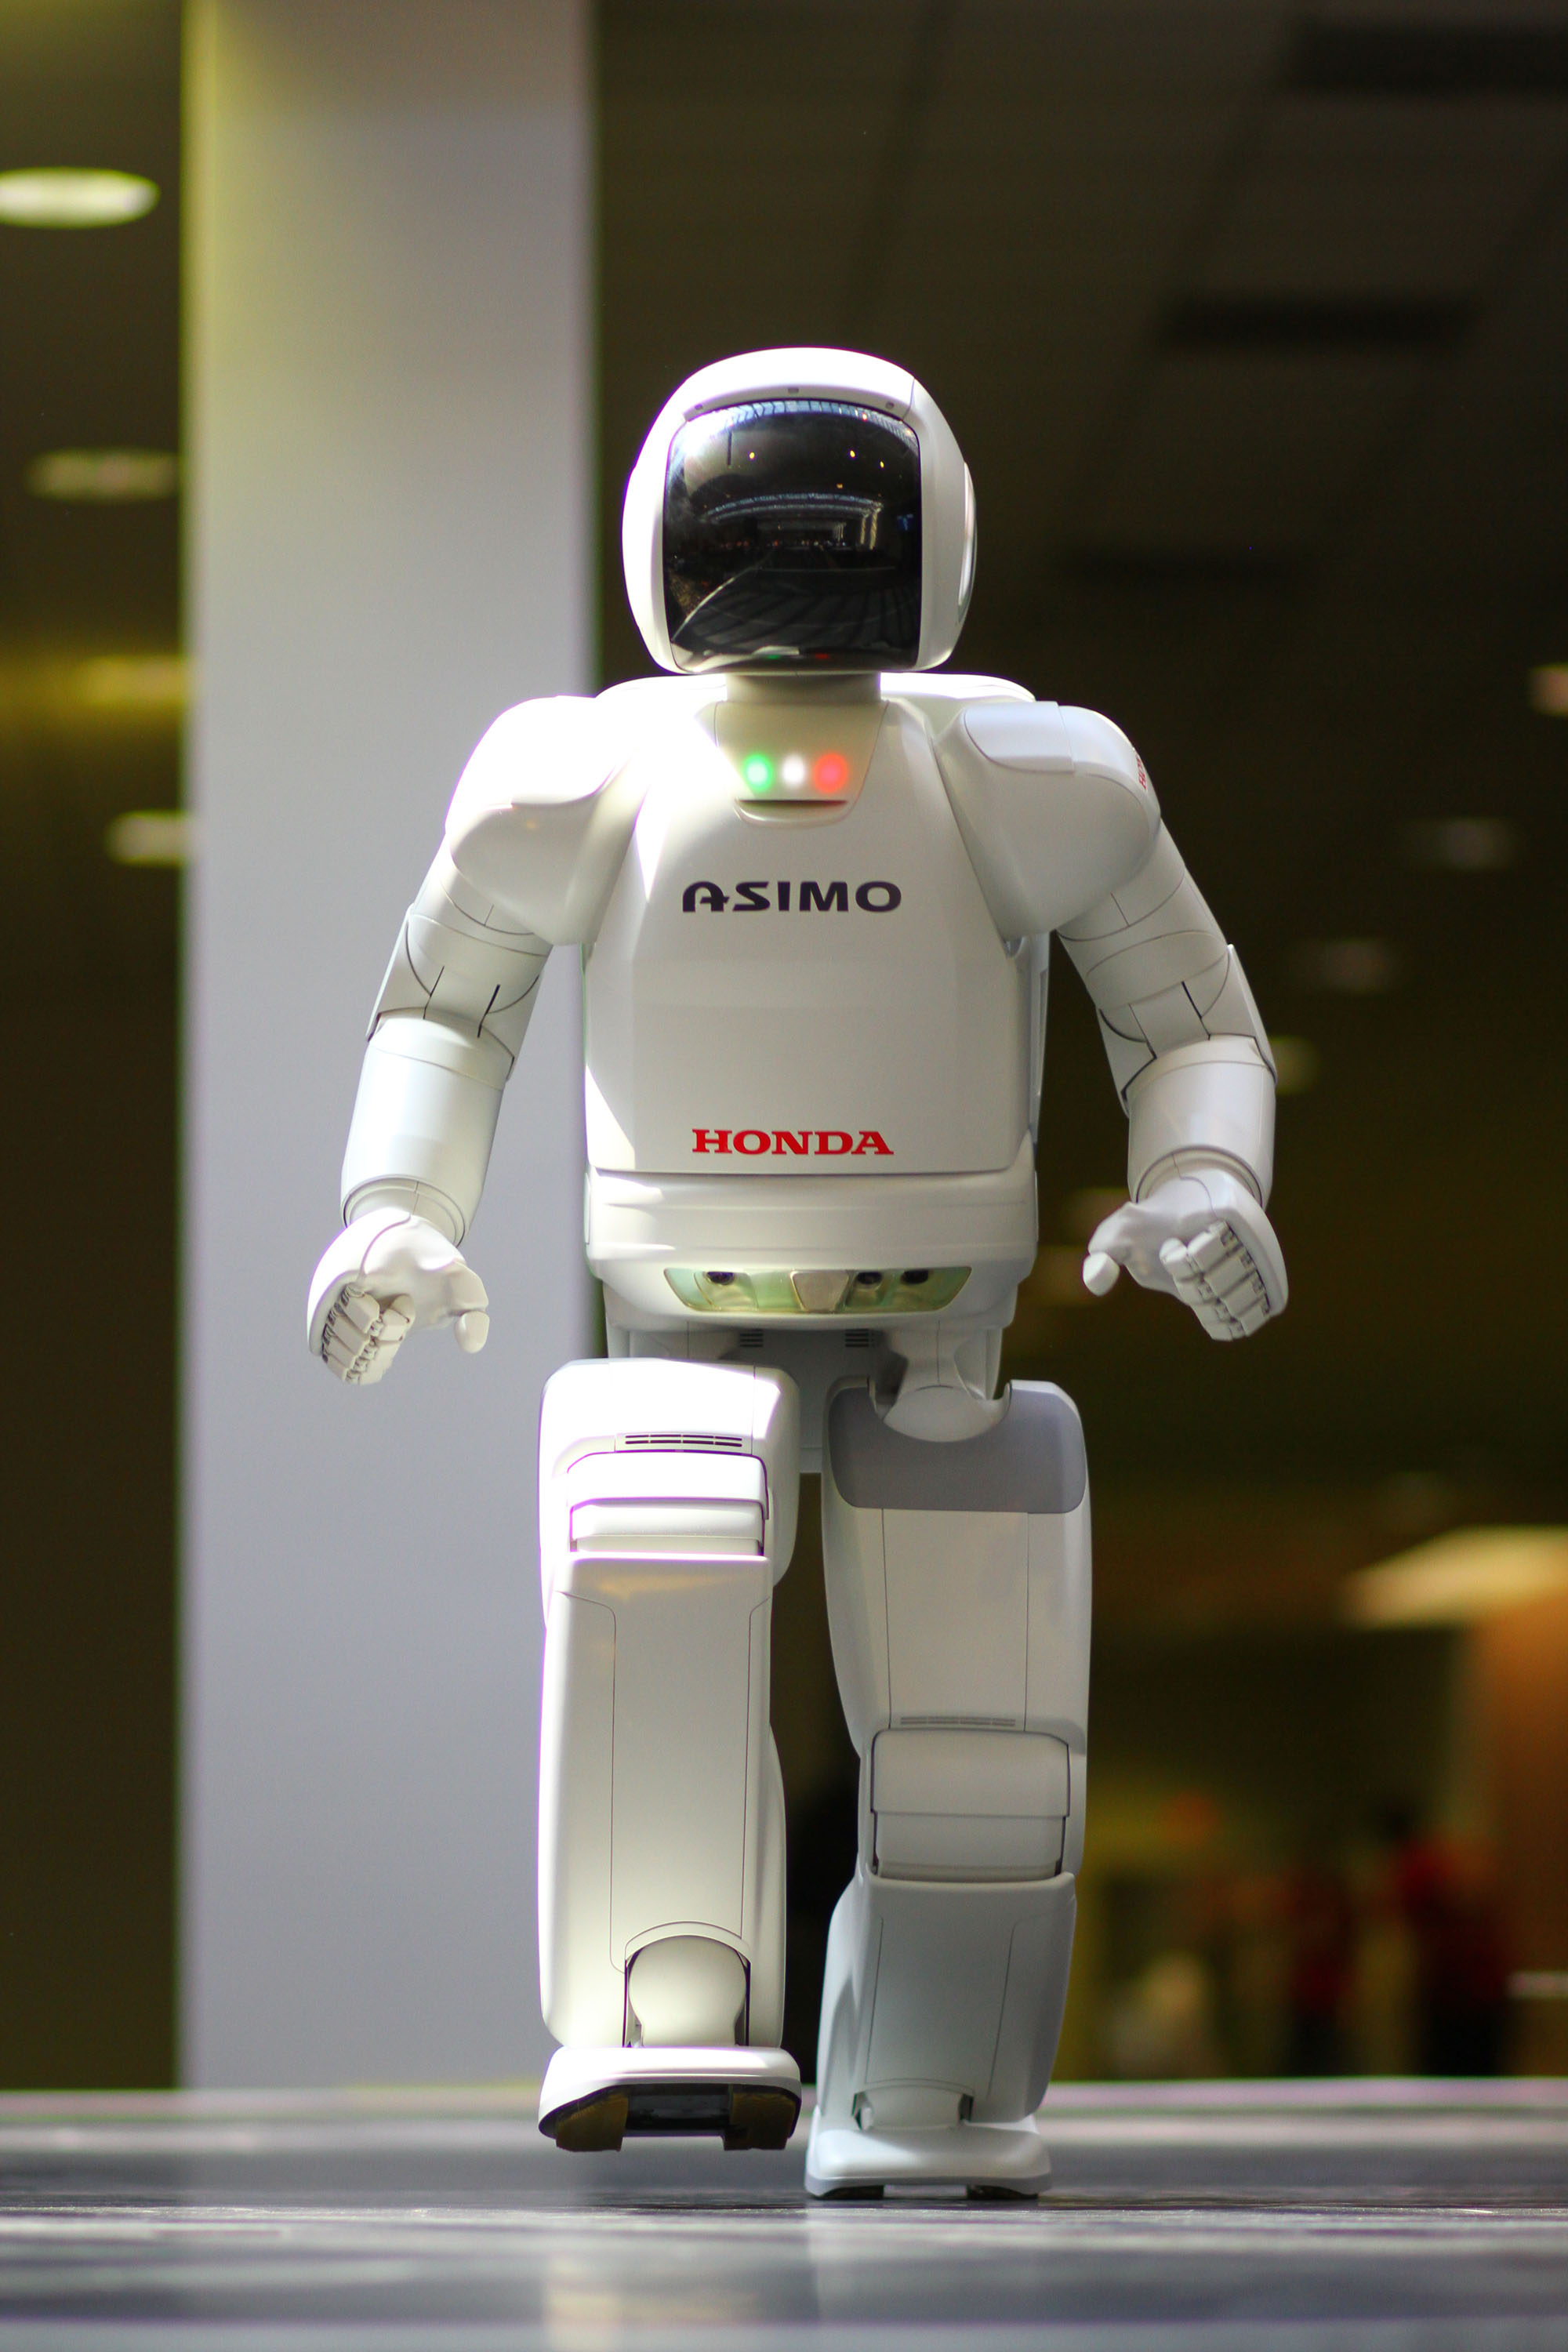
\includegraphics[scale=0.12]{./EtapaModerna/Imagenes/asimo.jpg}
	\caption{ASIMO \href{https://es.m.wikipedia.org/wiki/Archivo:ASIMO_4.28.11.jpg}{Wikimedia}}
\end{figure}
\end{frame}

%%%%%%%%%%%%%%%%%%%%%%%%%%%%%%%%%%%%%%%%%%%%%%%%%%%%%%%%%%%%%%%%%%%%%%%%%%%%%%%%%%%%%%%%%%%%%%
%%                                     Estado del Arte                                      %%
%%%%%%%%%%%%%%%%%%%%%%%%%%%%%%%%%%%%%%%%%%%%%%%%%%%%%%%%%%%%%%%%%%%%%%%%%%%%%%%%%%%%%%%%%%%%%%

\begin{frame}[fragile]{Estado del Arte}
\vspace{10px}
\pause
\metroset{block=fill}
\begin{block}{Principales Campos}
	\begin{itemize}
		\item NASA
		\pause
		\item Robots militares
		\pause
		\item Inteligencia Artificial
		\pause
		\item Robots Humanoides
	\end{itemize}
\end{block}
\end{frame}

%%%%%%%%%%%%%%%%%%%%%%%%%%%%%%%%%%%%%%%%%%%%%%%%%%%%%%%%%%%%%%%%%%%%%%%%%%%%%%%%%%%%%%%%%%%%%%
%%                                           NASA                                           %%
%%%%%%%%%%%%%%%%%%%%%%%%%%%%%%%%%%%%%%%%%%%%%%%%%%%%%%%%%%%%%%%%%%%%%%%%%%%%%%%%%%%%%%%%%%%%%%

\begin{frame}[fragile]{NASA}
\vspace{10px}
\pause
\metroset{block=fill}
\begin{block}{Brazos Robóticos}
	\begin{itemize}
		\item Robonaut, Dextre, Rassor
		\pause
		\item InSight y Mars 2020
		\pause
		\item Curiosity
	\end{itemize}
\end{block}
\begin{figure}
	\centering
	\pause
	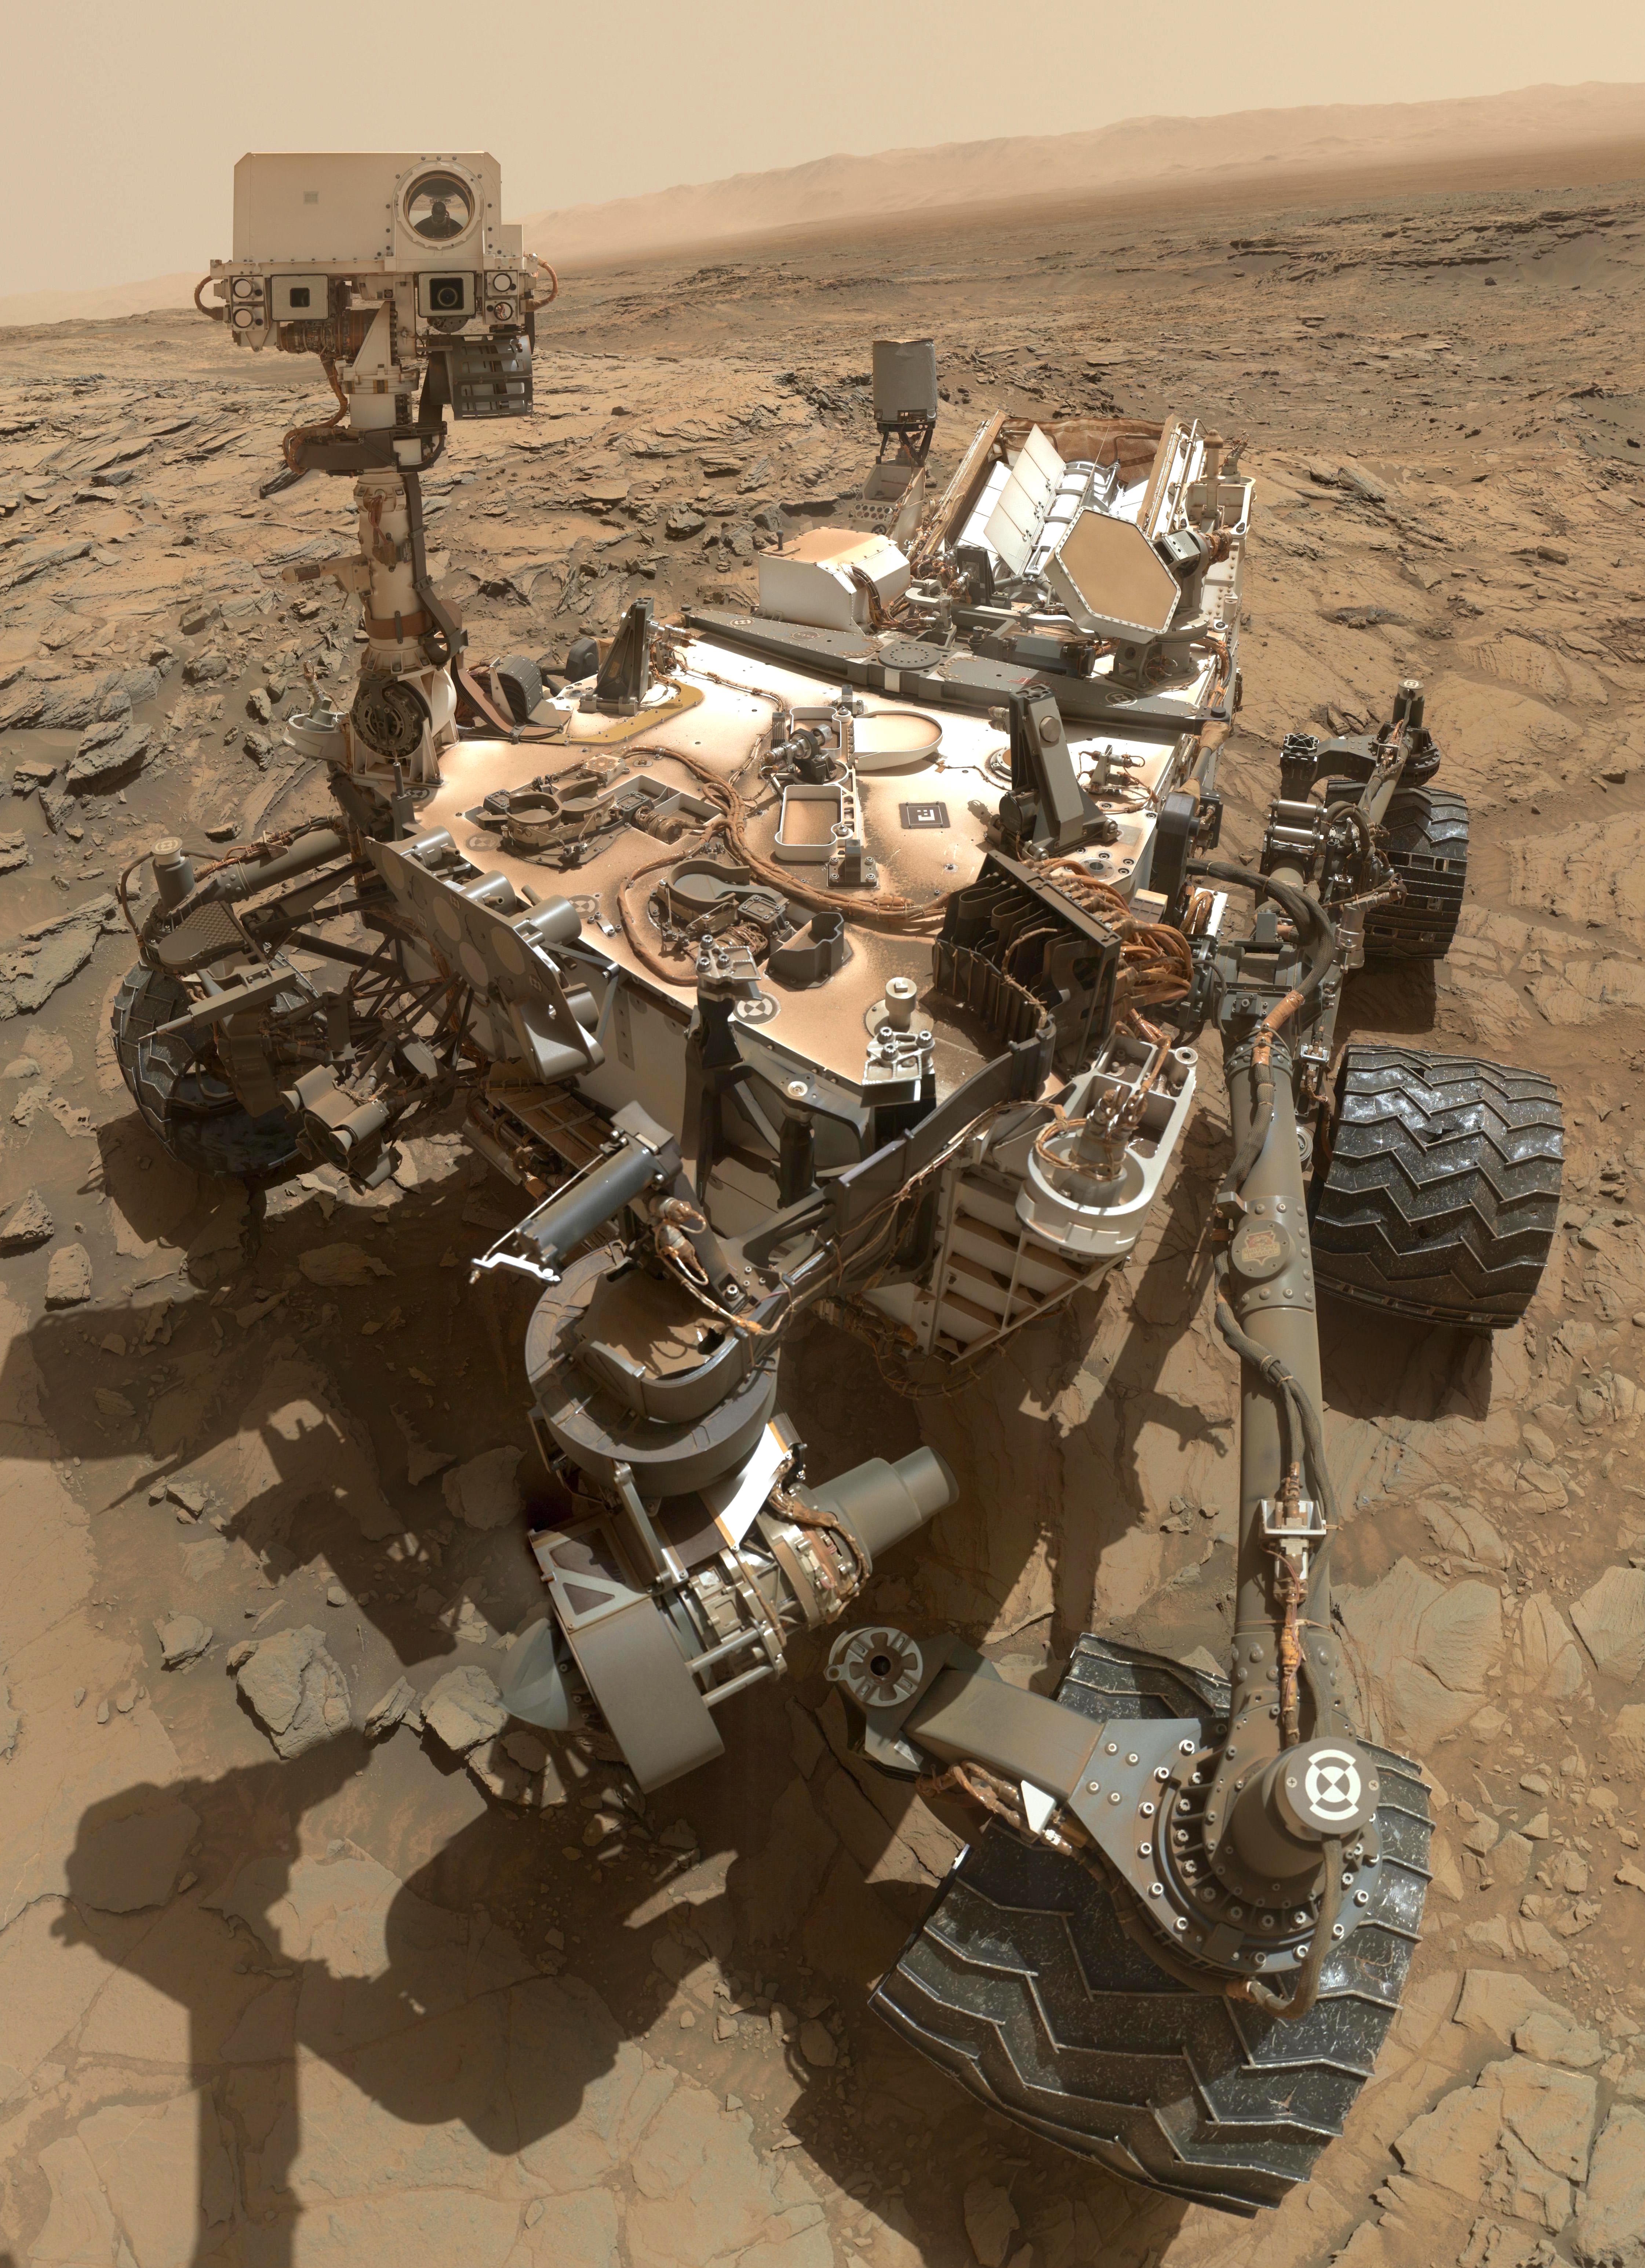
\includegraphics[scale=0.019]{./EtapaModerna/Imagenes/curiosity.jpg}
	\caption{Curiosity \href{https://en.wikipedia.org/wiki/File:Curiosity_Self-Portrait_at_\%27Big_Sky\%27_Drilling_Site.jpg}{Wikimedia}}
\end{figure}
\end{frame}

%%%%%%%%%%%%%%%%%%%%%%%%%%%%%%%%%%%%%%%%%%%%%%%%%%%%%%%%%%%%%%%%%%%%%%%%%%%%%%%%%%%%%%%%%%%%%%
%%                                     Robots militares                                     %%
%%%%%%%%%%%%%%%%%%%%%%%%%%%%%%%%%%%%%%%%%%%%%%%%%%%%%%%%%%%%%%%%%%%%%%%%%%%%%%%%%%%%%%%%%%%%%%

\begin{frame}[fragile]{Robots Militares}
\vspace{10px}
\pause
\metroset{block=fill}
\begin{block}{Robots Militares}
	\begin{itemize}
		\item Elbit Hermes 450
		\pause
		\item Guardium
		\pause
		\item TALON
		\pause
		\item SGR-A1
	\end{itemize}
\end{block}
\begin{figure}
	\centering
	\pause
	\centering
	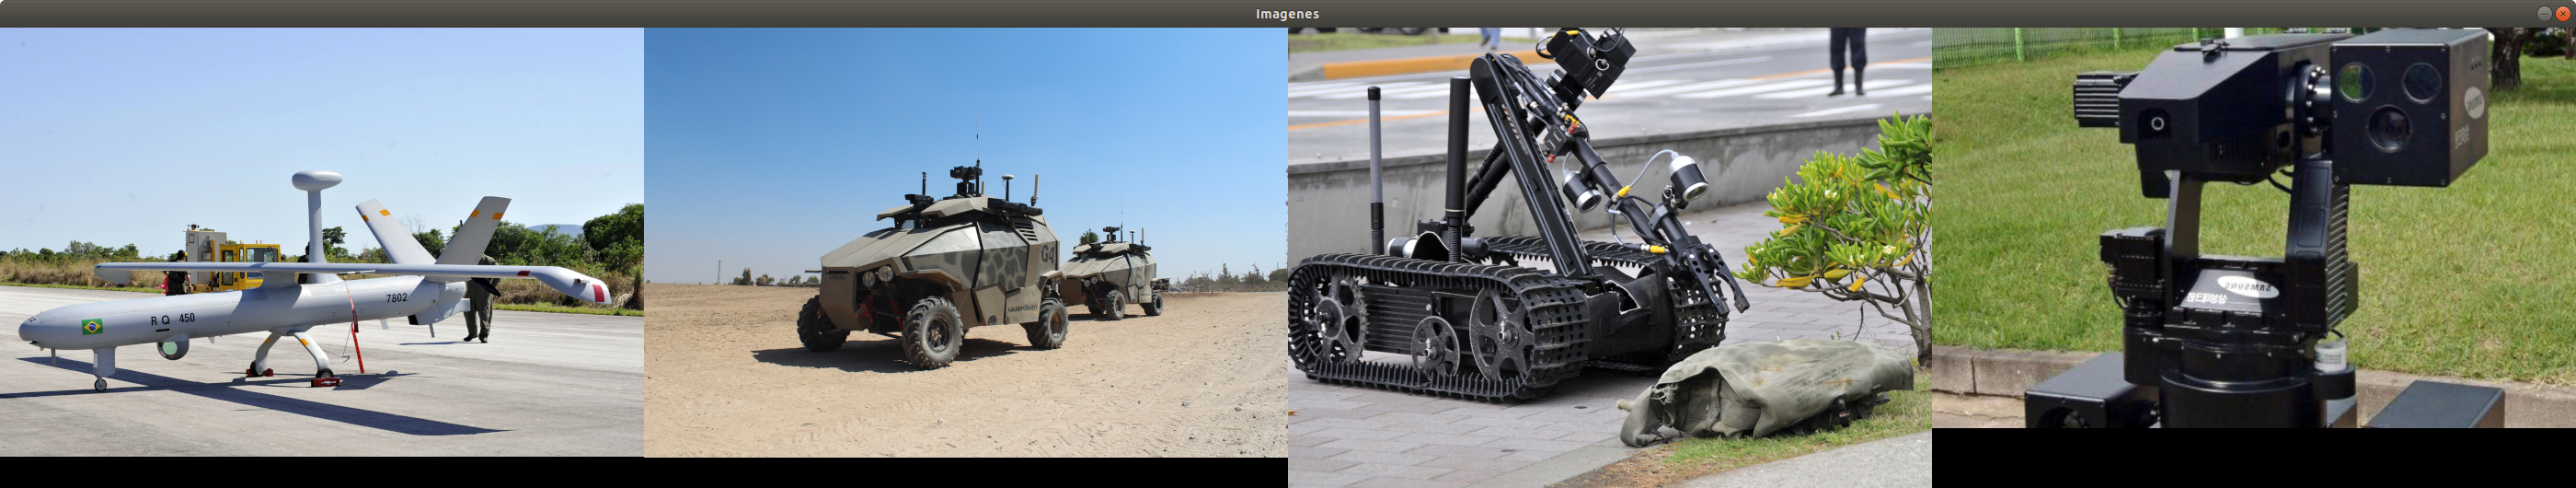
\includegraphics[scale=0.11]{./EtapaModerna/Imagenes/robots_militares.png}
	\caption{Elbit Hermes 450 \href{https://commons.wikimedia.org/wiki/File:Vant_Hermes_450_da_FAB_no_aeroporto_de_C\%C3\%A1ceres_(MT)_(8101398607).jpg}{Wikimedia}, Guardium \href{https://ca.wikipedia.org/wiki/Fitxer:Flickr_-_Israel_Defense_Forces_-_Israeli_Made_Guardium_UGV_(5).jpg}{Wikimedia}, TALON \href{https://commons.wikimedia.org/wiki/File:US_Navy_090512-N-2013O-013_A_Mark_II_Talon_robot_from_Explosive_Ordnance_Disposal_Mobile_Unit_5,_Det._Japan,_is_used_to_inspect_a_suspicious_package_during_a_force_protection-anti-terrorism_training_exercise.jpg}{Wikimedia}, SGR-A1 \href{https://commons.wikimedia.org/wiki/File:SGR-A1.jpg}{Wikimedia}}
\end{figure}
\end{frame}

%%%%%%%%%%%%%%%%%%%%%%%%%%%%%%%%%%%%%%%%%%%%%%%%%%%%%%%%%%%%%%%%%%%%%%%%%%%%%%%%%%%%%%%%%%%%%%
%%                                        Avances IA                                        %%
%%%%%%%%%%%%%%%%%%%%%%%%%%%%%%%%%%%%%%%%%%%%%%%%%%%%%%%%%%%%%%%%%%%%%%%%%%%%%%%%%%%%%%%%%%%%%%

\begin{frame}[fragile]{Avances de la IA}
\vspace{10px}
\pause
\metroset{block=fill}
\begin{block}{Sectores principales}
	\begin{itemize}
		\item Salud: Watson, brazos robóticos, prótesis, ...
		\pause
		\item Automoción: conducción inteligente y asistencia.
		\pause
		\item Economía: análisis de la banca y operaciones en bolsa.
		\pause
		\item Publicidad: más efectiva.
	\end{itemize}
\end{block}
\begin{figure}
	\centering
	\pause
	\begin{subfigure}{0.45\textwidth}
		\centering
		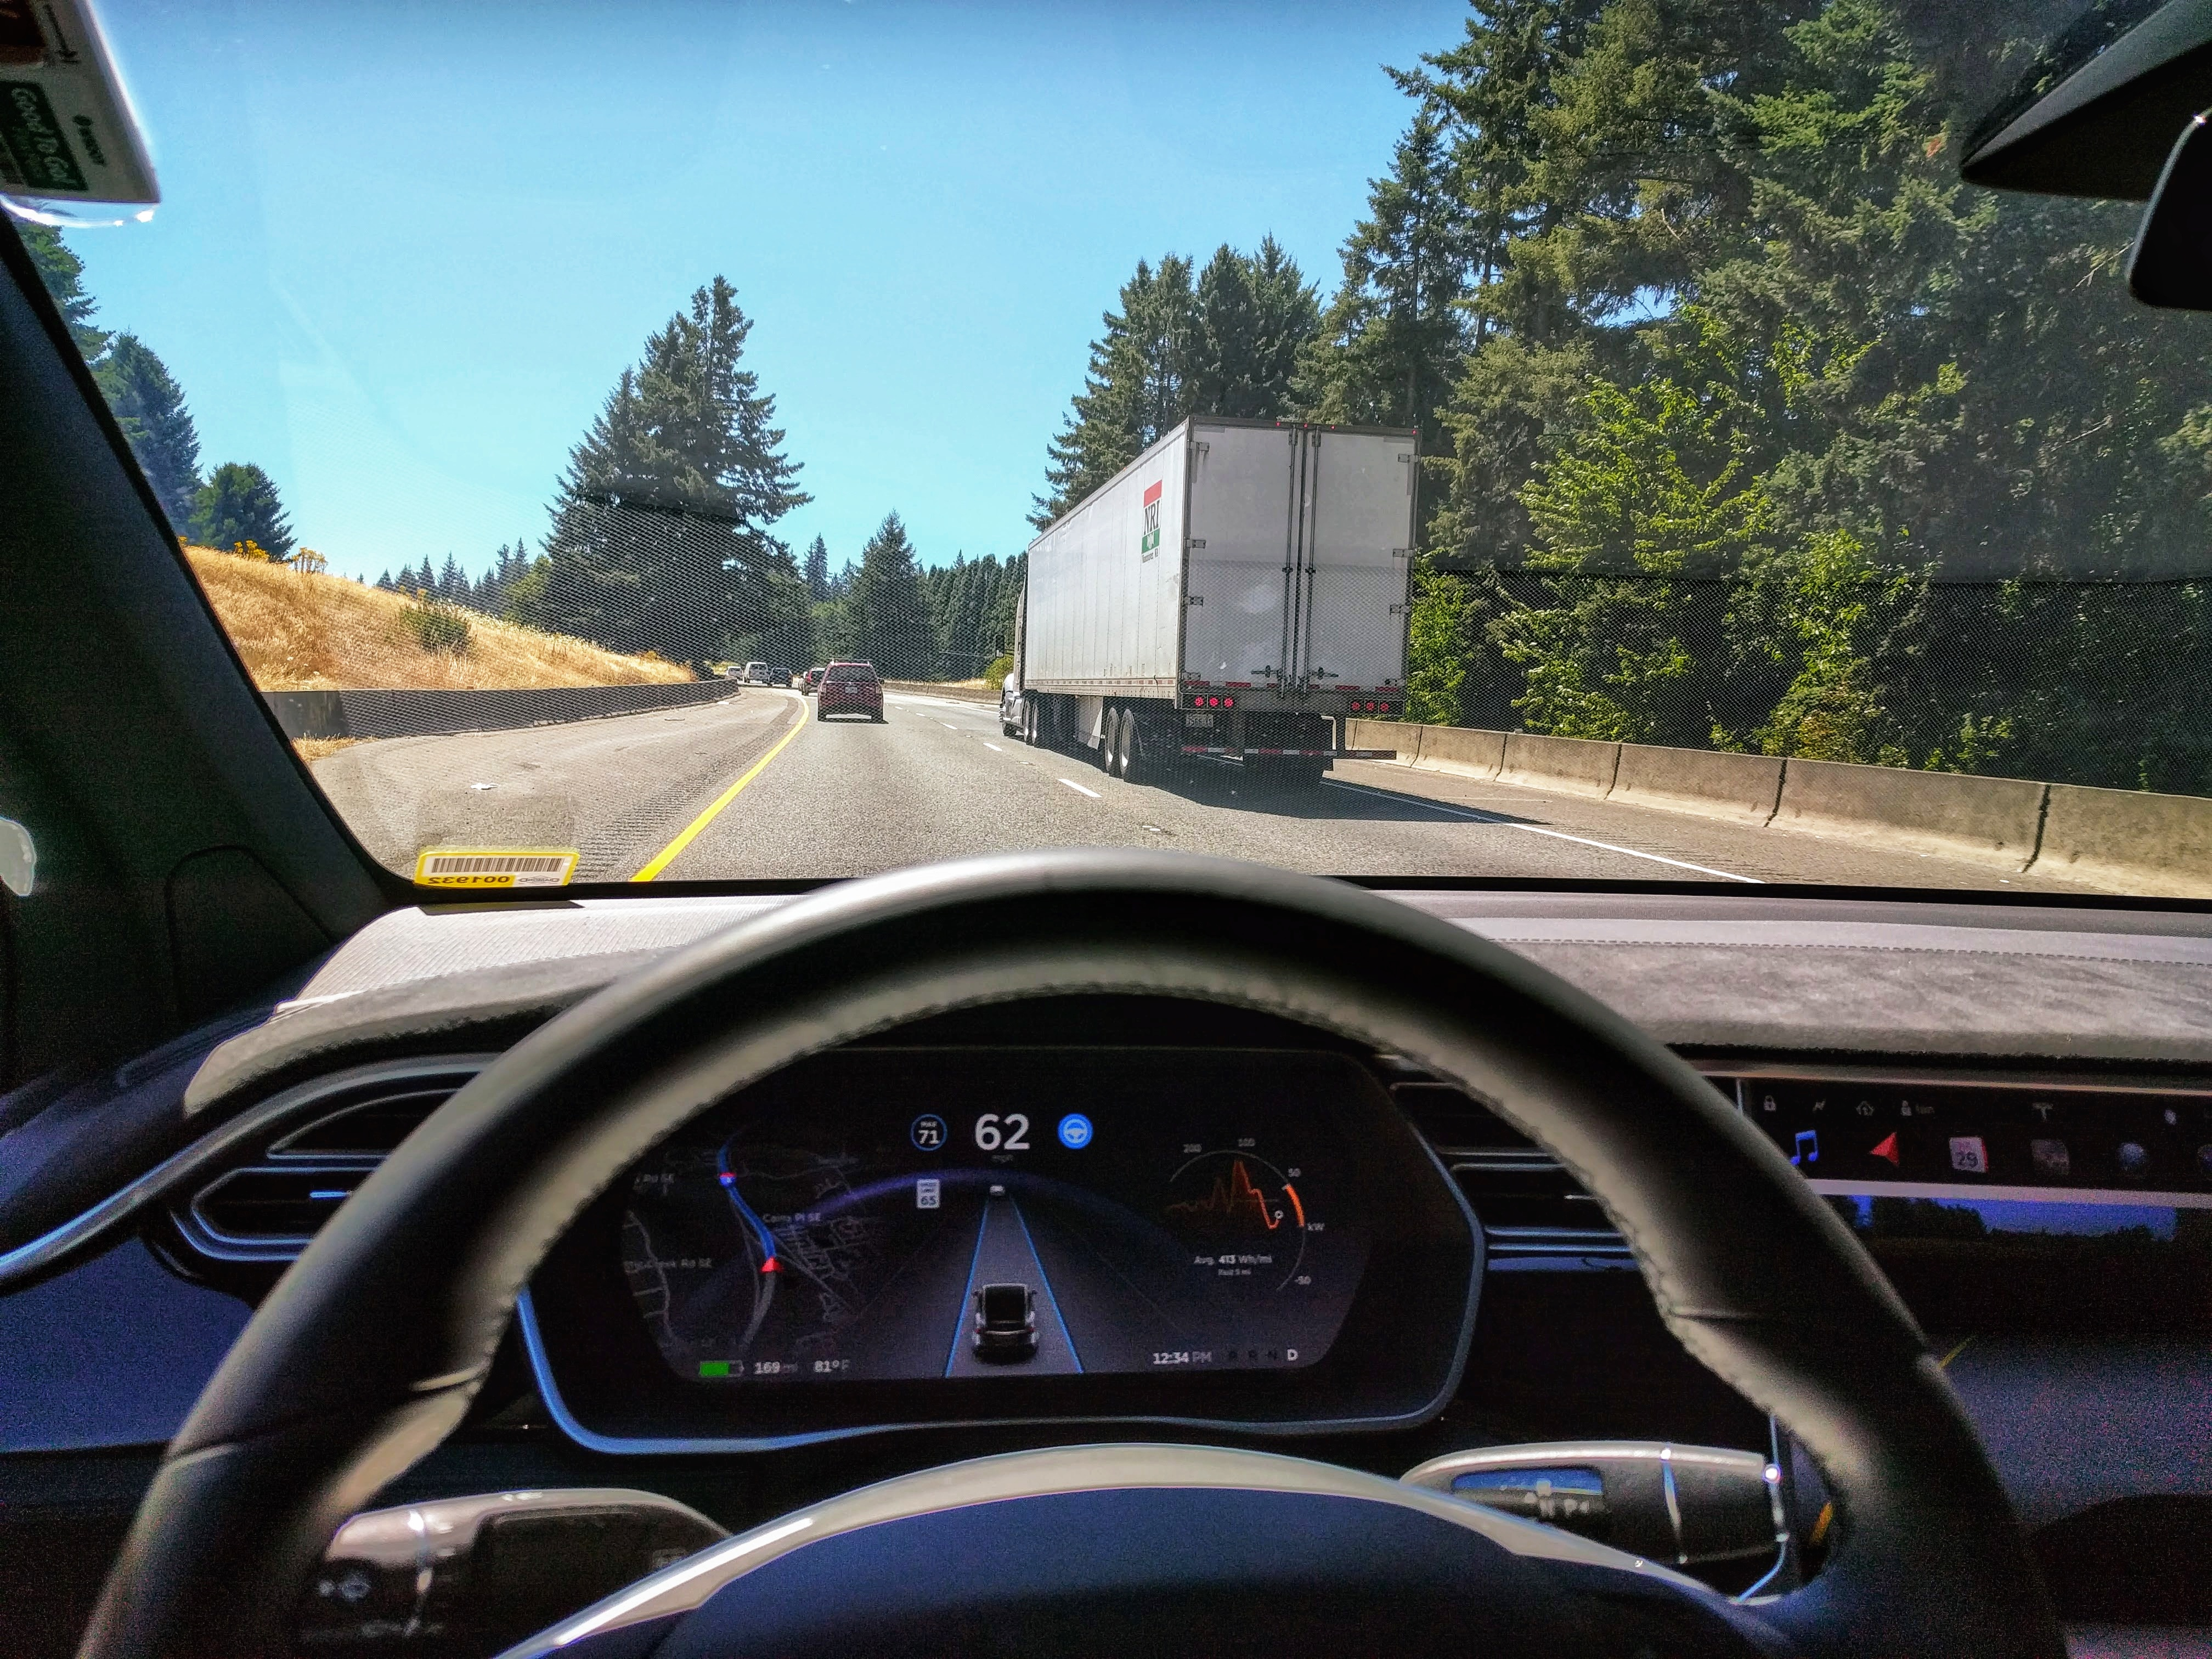
\includegraphics[scale=0.025]{./EtapaModerna/Imagenes/autopilot.jpg}
		\caption{Autopilot \href{https://commons.wikimedia.org/wiki/File:Tesla_Autopilot_Engaged_in_Model_X.jpg}{Wikimedia}}
	\end{subfigure}
	\pause
	\begin{subfigure}{0.45\textwidth}
		\centering
		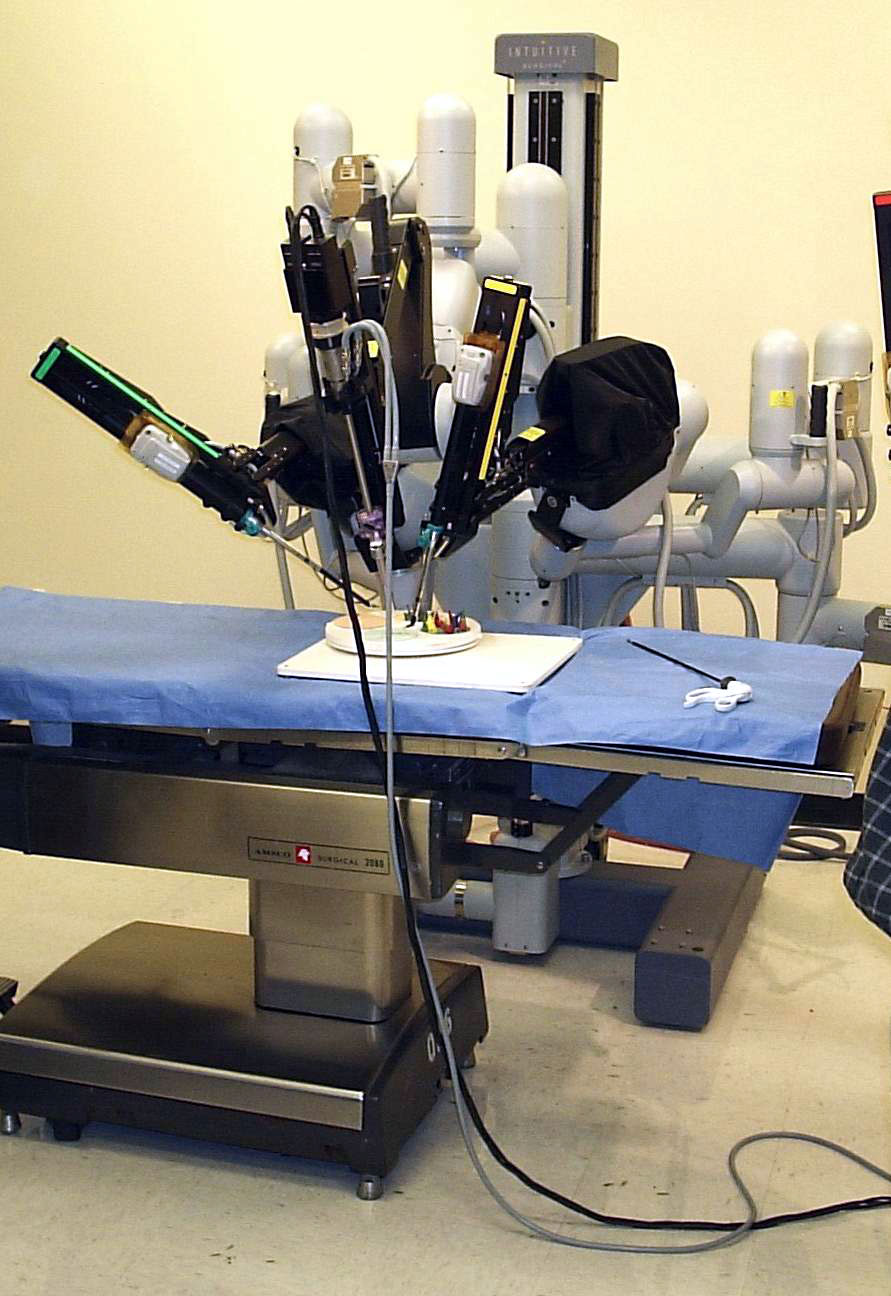
\includegraphics[scale=0.07]{./EtapaModerna/Imagenes/robot_surgery.jpg}
		\caption{Robot para laparoscopia \href{https://es.m.wikipedia.org/wiki/Archivo:Laproscopic_Surgery_Robot.jpg}{Wikimedia, por Nimur}}
	\end{subfigure}
\end{figure}
\end{frame}

%%%%%%%%%%%%%%%%%%%%%%%%%%%%%%%%%%%%%%%%%%%%%%%%%%%%%%%%%%%%%%%%%%%%%%%%%%%%%%%%%%%%%%%%%%%%%%
%%                                    Robots Humanoides                                     %%
%%%%%%%%%%%%%%%%%%%%%%%%%%%%%%%%%%%%%%%%%%%%%%%%%%%%%%%%%%%%%%%%%%%%%%%%%%%%%%%%%%%%%%%%%%%%%%

\begin{frame}[fragile]{Robots Humanoides}
\vspace{10px}
\pause
\metroset{block=fill}
\begin{block}{Principales Robots}
	\begin{itemize}
		\item Actroid: asistente por voz sencillo.
		\pause
		\item Wakamaru: robot para las casas.
		\pause
		\item iCub: imitación de movimientos humanos complejos.
		\pause
		\item Sophia: interacción oral y gestual. Gestión de las emociones.
	\end{itemize}
\end{block}
\begin{figure}
	\centering
	\pause
	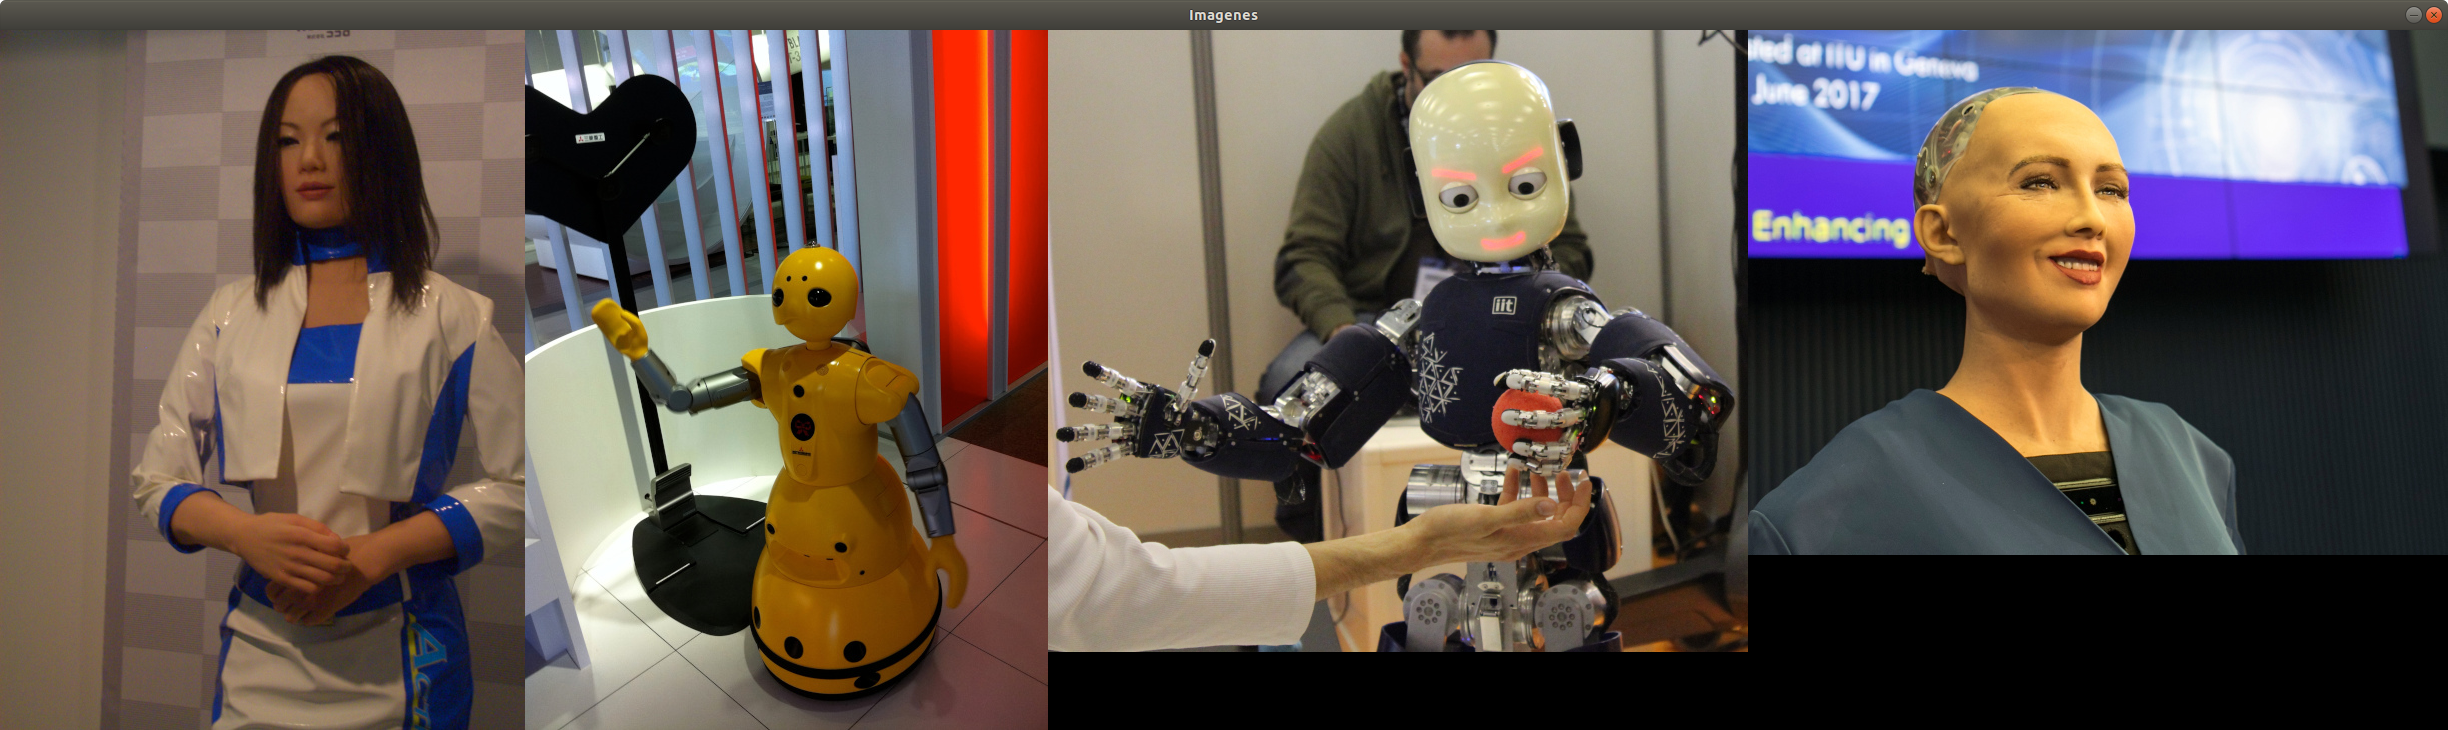
\includegraphics[scale=0.12]{./EtapaModerna/Imagenes/robots_humanoides.png}
	\caption{Actroid \href{https://commons.wikimedia.org/wiki/File:Actroid_3.jpg}{Wikimedia}, Wakamaru \href{https://commons.wikimedia.org/wiki/File:Wakamaru-fullshot2011.jpg}{Wikimedia}, iCub \href{https://commons.wikimedia.org/wiki/File:ICub_Innorobo_Lyon_2014.JPG}{Wikimedia}, Sophia \href{https://es.wikipedia.org/wiki/Archivo:Sophia_(robot).jpg}{Wikimedia}}
\end{figure}
\end{frame}